\documentclass[12pt]{article}

\usepackage[hmargin=2.5cm, vmargin={3cm,3cm}, a4paper]{geometry} 
\usepackage{amsmath,amssymb,amsthm,mathrsfs}
\usepackage{epsfig,epsf,subfigure,graphicx,graphics}
\usepackage{float}
\usepackage{url,enumerate}
\usepackage{listings}
\usepackage{ragged2e}
\graphicspath{{fig/}}
\usepackage{fancyhdr}
\usepackage{hyperref}
\hypersetup{
    colorlinks=true,
    linkcolor=blue,
    filecolor=magenta,      
    urlcolor=cyan,
    pdfpagemode=FullScreen,
    }
\setlength{\headheight}{12pt}
\pagestyle{fancyplain}

\graphicspath{ {./images/} }%Path to the images
 
\rhead{}
\lhead{}
\chead{{\it Graph Signal Processing Course, ETSETB}}
\lfoot{}
\cfoot{\thepage}
\rfoot{}
\title{Practical session 3: Graph Filtering}
\author{Gerard Castell and Victor Rubio}
\begin{document}
\maketitle

\thispagestyle{fancyplain}
\flushleft 


\Large
\hspace{10pt}
\small
\section{US Weather Station}

%%Abstract Subsection
\subsection{Abstract}
\justifying
In this practice we have constructed several graph filters to evaluate the temperature from 200 stations during 365 days in the U.S in the 2002. Such stations are connected geographically with the 8 closest stations. In addition, it is also provided the position of the stations so we are able to build a graph and we know the connections, i.e. edges, of each one. So the target of this session is to apply a low and a high-pass filter for different day of each season and obtain the graph with the applied filtered signals.
%%First subsection
\subsection{Reading and visualization of the data}
\justifying
To perform this experiment we have retrieved three matrices from the dataset.
\begin{itemize}
    \item \textbf{Y}. It is the vector which contains the temperature in Fahrenheit degrees of the 200 stations along 365 days. So it is a matrix of 200x365. In order to ease the understanding of the plots it has been transformed to Celsius degrees.
    \item \textbf{A}. It is the adjacency matrix of the graph that relates the stations and how they are connected. Hence, its dimensions are 200x200.
     \item \textbf{pos}. It defines the position of the stations in geographical coordinates, so it is 200x2.
\end{itemize}


%Second subsection
\subsection{Generation of an undirected graph}
\justifying Thanks to the data explained in the previous section we are able to build a graph. The resulting image is the following.

\begin{figure}[H]
	\centering
	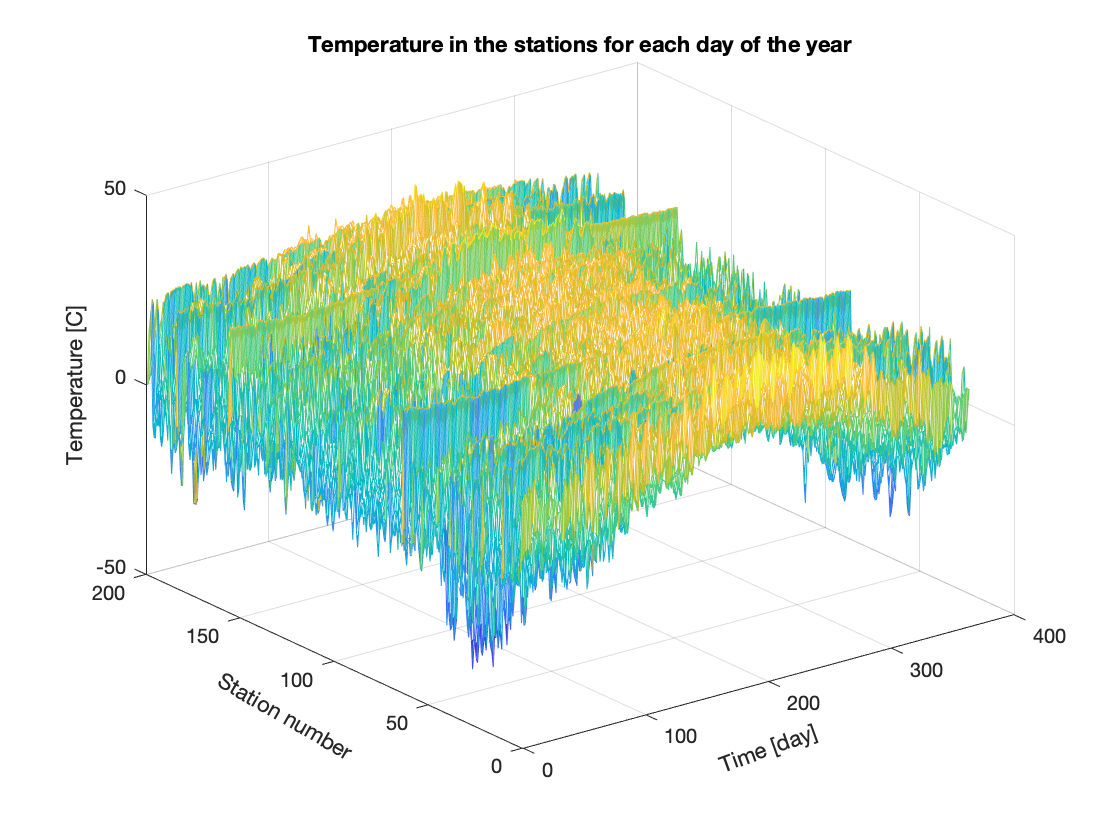
\includegraphics[width=13cm]{images/1.png}
	\caption{Plot of the temperature per station during a whole year.}
	\label{fig:temperaturePlot}
\end{figure}

With that information we were able to build a directed graph such as this:
\begin{figure}[H]
	\centering
	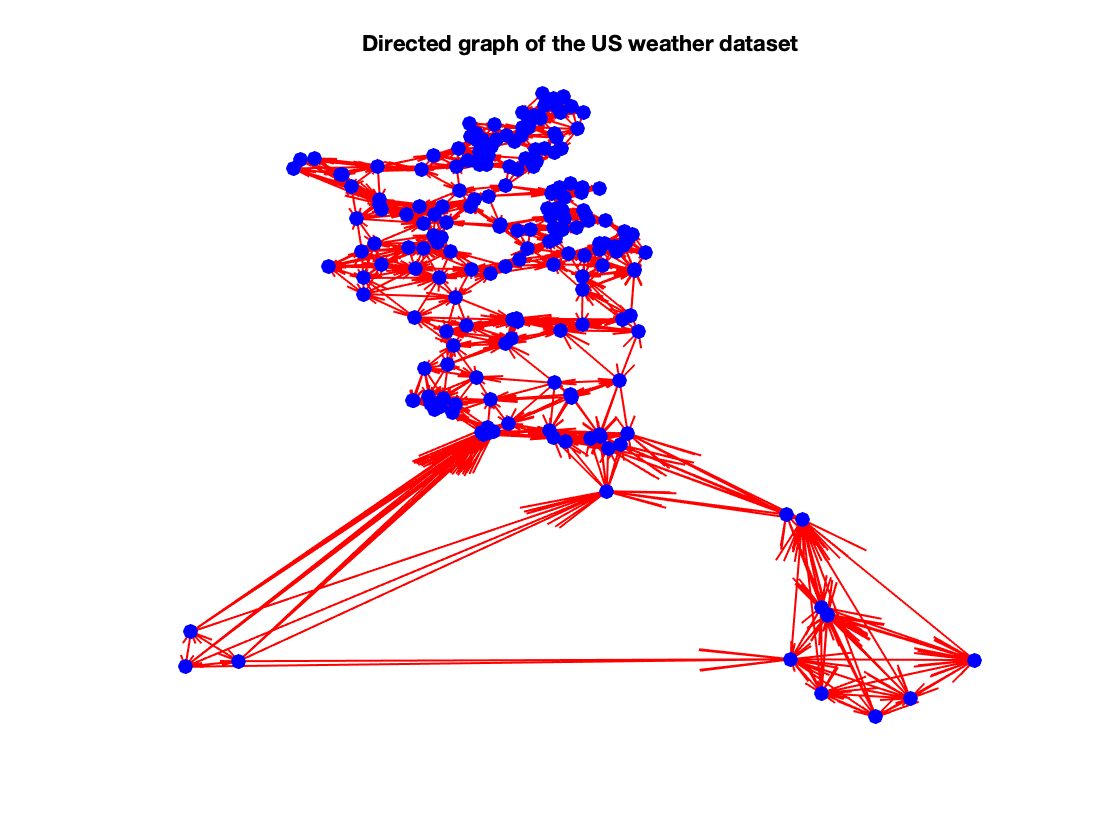
\includegraphics[width=13cm]{images/2.png}
	\caption{Plot of the directed graph of the stations.}
	\label{fig:directedGraph}
\end{figure}

After that, we have looked for the Hawaii stations and removed the three entries related to that coordinates. The resulting graph is the following:

\begin{figure}[H]
	\centering
	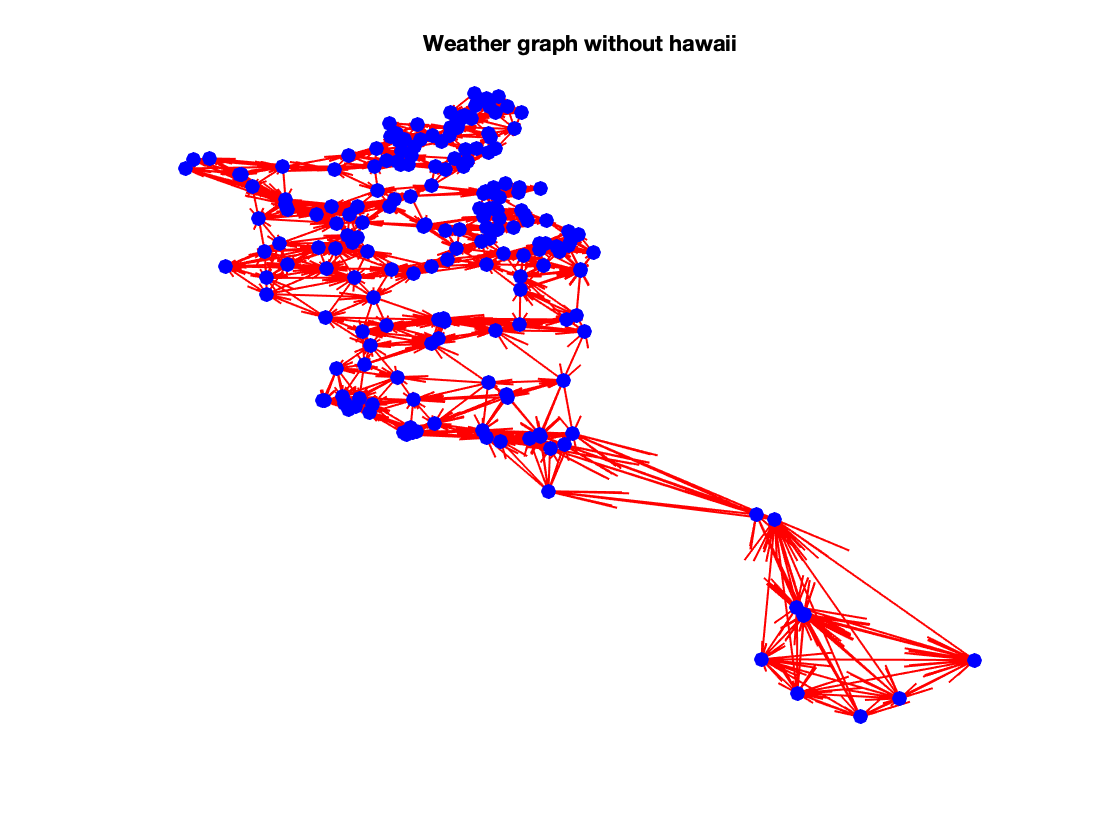
\includegraphics[width=10cm]{images/3.png}
	\caption{Plot of the directed graph removing Hawaii entries.}
	\label{fig:excludedHawaiiGraph}
\end{figure}

As you can see if you compare the graph \ref{fig:directedGraph} with the previous one \ref{fig:excludedHawaiiGraph}, we can see how the nodes at the south-west corner has been erased. So they are not going to be considered in the experiment. Finally, we have converted the graph to undirected in order to simplify the calculations.

\begin{figure}[H]
	\centering
	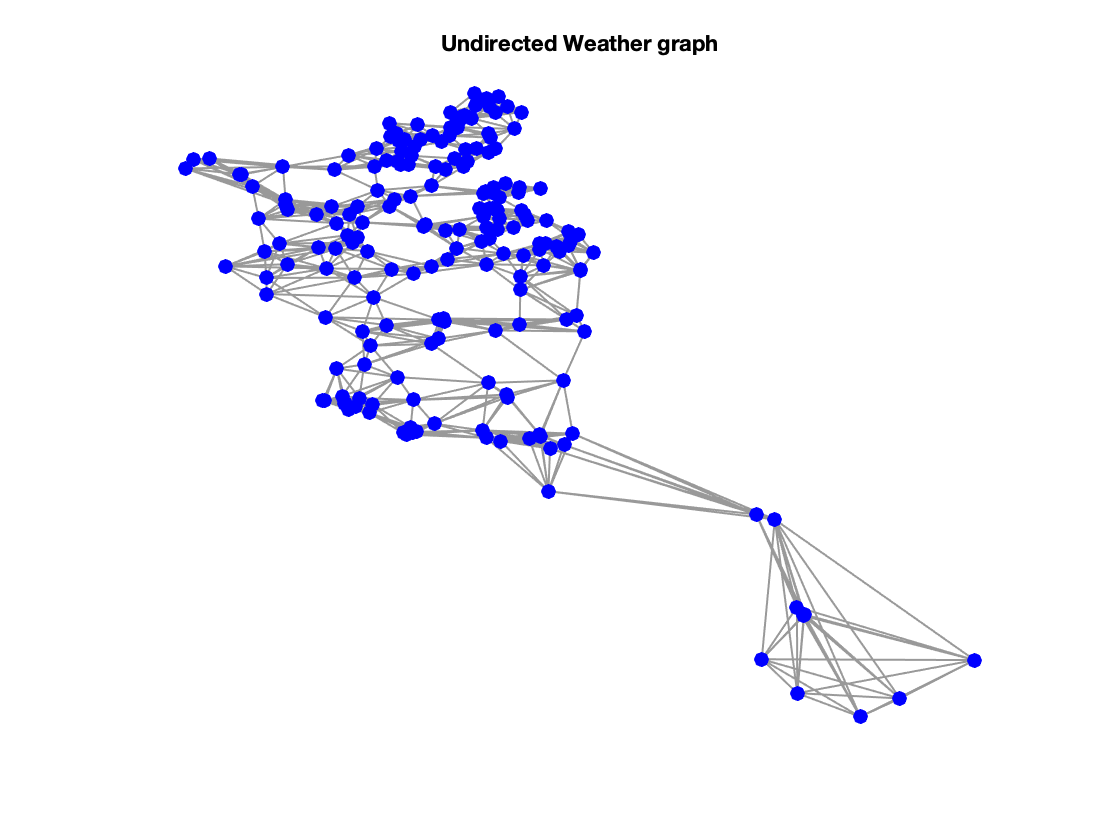
\includegraphics[width=10cm]{images/4.png}
	\caption{Plot of the directed graph removing Hawaii entries.}
	\label{fig:undirectedGraph}
\end{figure}

%Third subsection
\subsection{Low pass filter}
\justifying
We have developed a filter function with the aim of given a Graph, a filter function, which will depend of it purpose, and an input signal. As output it returns the resulting filtered signal. $filter(G,x, h)$:
\label{code:CNScoring}
\begin{lstlisting}
function y = filter(G,x, h)
    x_hat = G.U' * x;
    y_hat_l = h.*x_hat;
    y = G.U*y_hat_l;
end
\end{lstlisting}
\justifying

So we have selected a random day and we have computed the Graph Fourier Basis with the function $gsp\_compute\_fourier\_basis(G_u)$, where $G_u$ is the undirected graph without Hawaii stations.
The low pass filter has been calculated as this: $\tilde{h}_l= 1/(1+G_u.e)$
The resulting plot that compares the input signal in the graph with the low pass filter is this:
\begin{figure}[H]
	\centering
	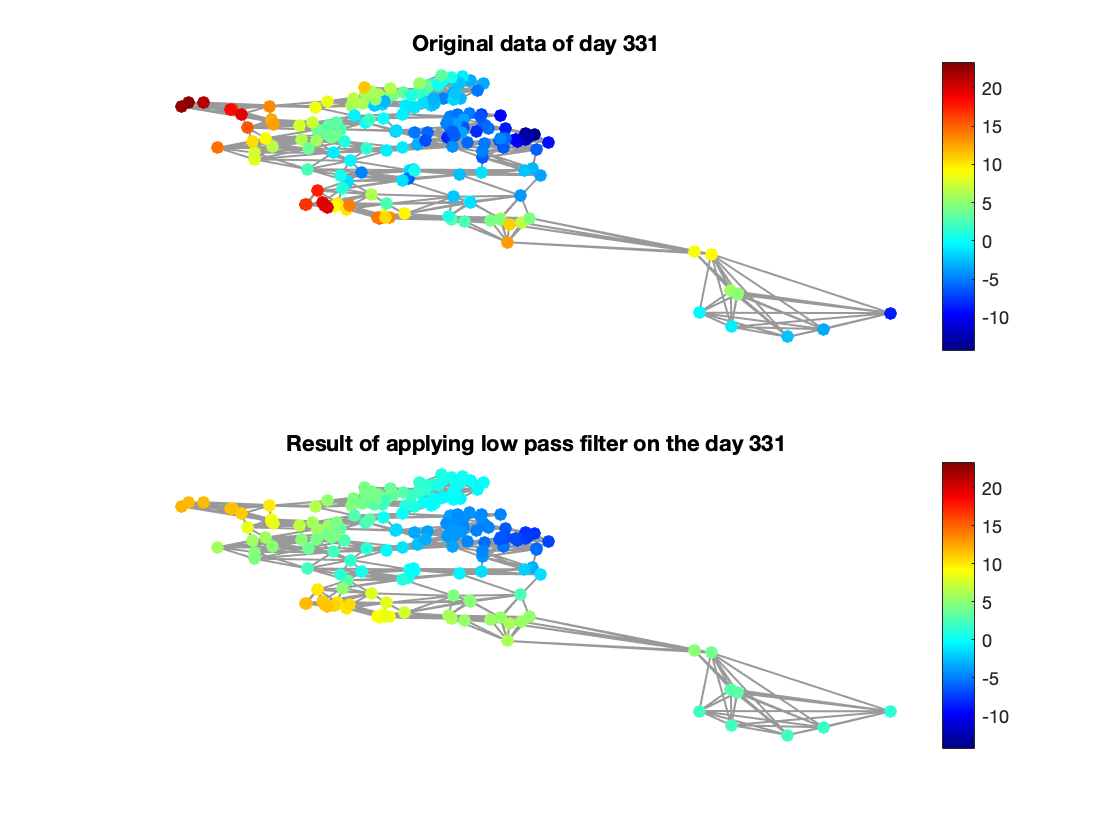
\includegraphics[width=13cm]{images/5.png}
	\caption{Plot of the low pass filter graph compared with the original input signal.}
	\label{fig:lowpassfilterrandom}
\end{figure}

As we may observe in the plot, the temperatures across the graph does not have heavy variations, keeping the lowest temperature nodes. If we focus on the right-side nodes we can see how the temperature propagates to the left nodes without changing the temperature that sudden as the original signal.
%4th subsection
\subsection{High pass filter}
\justifying
For this purpose we have used the previous function $filter(G,x, h)$ but this time with the High pass filter definition $\tilde{h}_h= 1/(1-(G_u.e-\lambda_{max}))$. Applying such a filter to the same input signal than before we obtain this representation.
\begin{figure}[H]
	\centering
	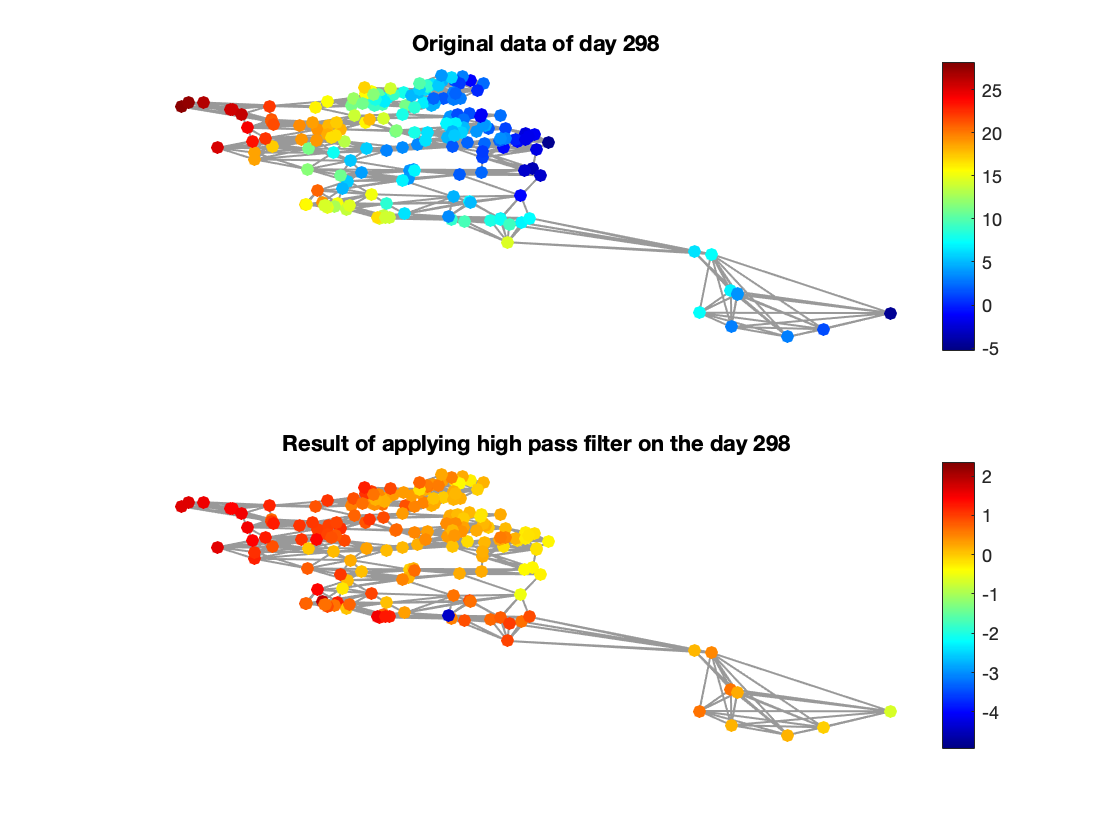
\includegraphics[width=10cm]{images/6.png}
	\caption{Plot of the high pass filter graph compared with the original input signal.}
	\label{fig:lowpassfilterrandom}
\end{figure}
On the other hand, the whole graph contains  red, orange and yellow nodes, and we can see that the interval of values that are represented in the graph is from -4 to 2 degrees Celsius. This means that the high-pass filter will remove the temperature information from the data and maintain the noise from the data. What is represented then, is mostly the noise.

\subsection{High and low pass filter per season }
For the final part, we have plot a random day for each season in order to see how the filters works for each stage of the year.
\begin{figure}[H]
	\centering
	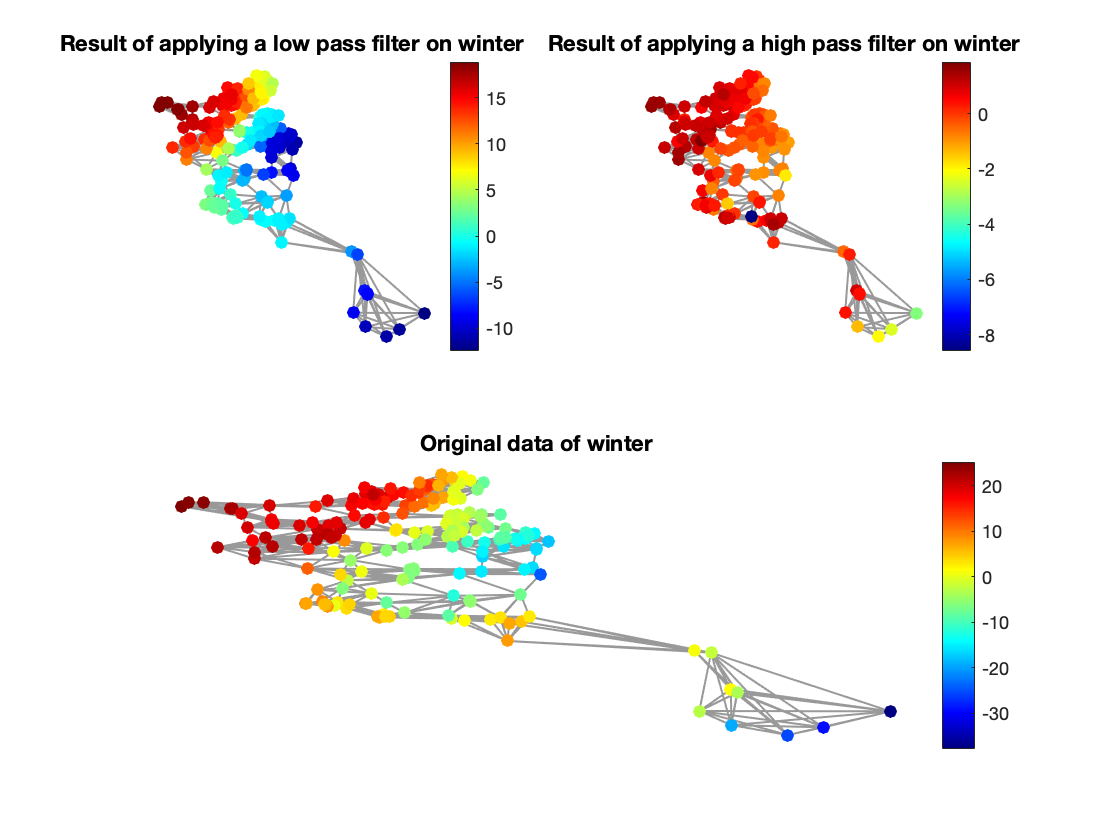
\includegraphics[width=10cm]{images/7.png}
	\caption{Plot of the high pass filter graph compared with the original input signal.}
	\label{fig:lowpassfilterrandom}
\end{figure}
\begin{figure}[H]
	\centering
	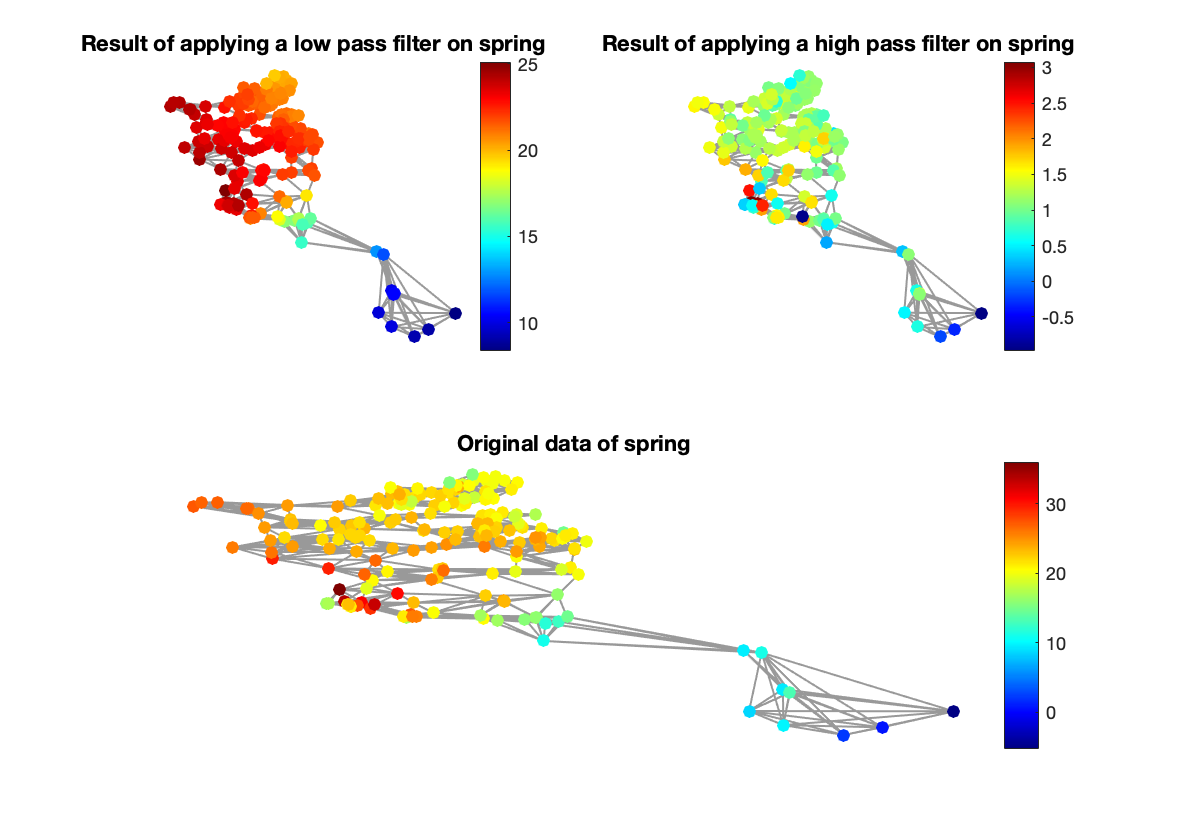
\includegraphics[width=10cm]{images/8.png}
	\caption{Plot of the high pass filter graph compared with the original input signal.}
	\label{fig:lowpassfilterrandom}
\end{figure}
\begin{figure}[H]
	\centering
	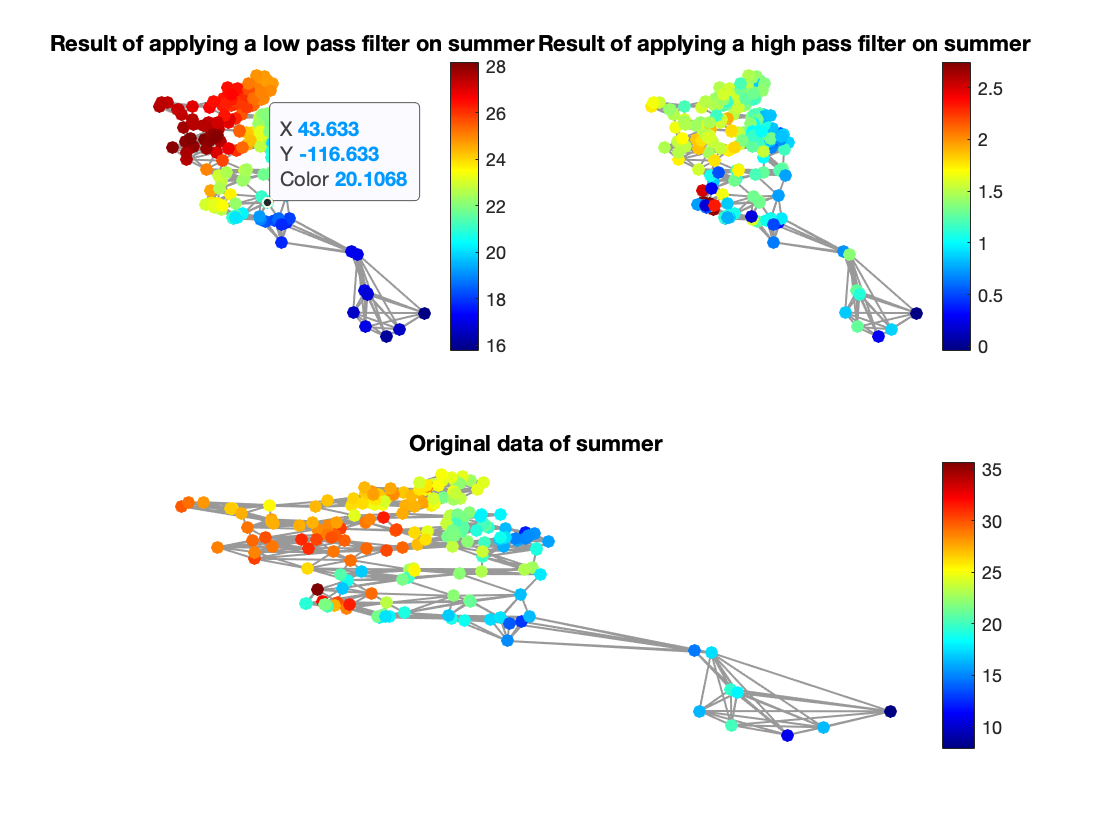
\includegraphics[width=10cm]{images/9.png}
	\caption{Plot of the high pass filter graph compared with the original input signal.}
	\label{fig:lowpassfilterrandom}
\end{figure}
\begin{figure}[H]
	\centering
	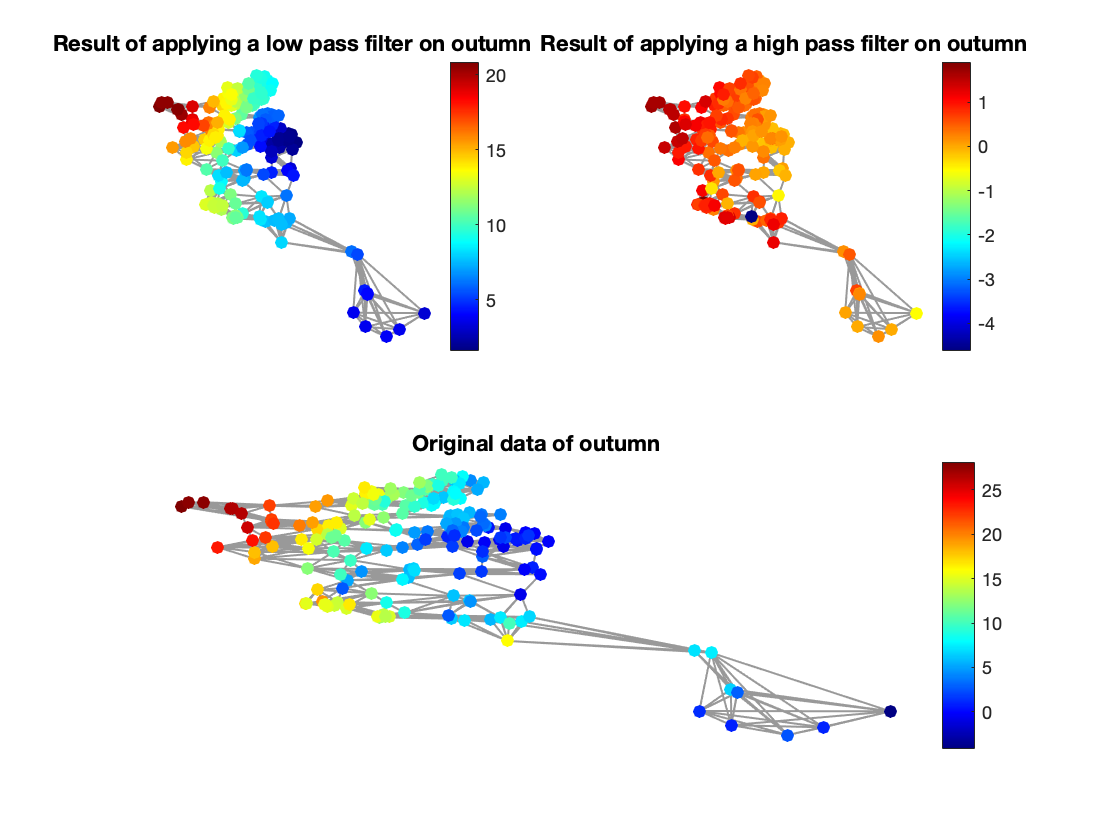
\includegraphics[width=10cm]{images/10.png}
	\caption{Plot of the high pass filter graph compared with the original input signal.}
	\label{fig:lowpassfilterrandom}
\end{figure}
In the previous images we can see that the temperatures in have a great variation in the original data, as it is in the United States of America and the country is huge. Therefore, it is normal that the temperature in the different places is extremely different. In this sense, using a low pass filter will help us keep the most relevant data and we well see a decrease in the range values of the legend, thus helping us getting the most relevant information. The graph will turn out to be more smooth, due to the effect of the low-pass filter.

Applying the high-pass filter will remove the temperature information in the lowest frequencies and mostly noise will remain.

\end{document}
